%%% Preample
\documentclass[aps,prl,reprint,superscriptaddress,floatfix]{revtex4-1}
\usepackage[utf8]{inputenc}

\usepackage{amsmath,amssymb,upgreek}
\usepackage{physics}
\usepackage{braket}
\usepackage{esvect}
%\usepackage{wasysym}
\usepackage{gensymb}
\usepackage{textcomp}

\usepackage[pdftex]{graphicx}
\graphicspath{{../Figures/}}
\DeclareGraphicsExtensions{.pdf,.jpeg,.png,.jpg}
\usepackage{hyperref}

\usepackage{xcolor}

\usepackage{soul}

\usepackage{lipsum}
\usepackage{pdfcomment}

%%% Begin document
\begin{document}

%%% Title
\title{The \textit{spider web} array--a sparse spin qubit array}
\date{\today}

%%% Authors and affiliations
\author{Jelmer M. Boter}
\affiliation{QuTech, Delft University of Technology, Lorentzweg 1, 2628 CJ Delft, The Netherlands}
\affiliation{Kavli Institute of Nanoscience, Delft University of Technology, Lorentzweg 1, 2628 CJ Delft, The Netherlands}

\author{Juan P. Dehollain}
\affiliation{QuTech, Delft University of Technology, Lorentzweg 1, 2628 CJ Delft, The Netherlands}
\affiliation{Kavli Institute of Nanoscience, Delft University of Technology, Lorentzweg 1, 2628 CJ Delft, The Netherlands}
\affiliation{School of Mathematical and Physical Sciences, University of Technology Sydney, Ultimo NSW 2007, Australia}

\author{Jeroen P.~G. van Dijk}

\author{Toivo Hensgens}
\affiliation{QuTech, Delft University of Technology, Lorentzweg 1, 2628 CJ Delft, The Netherlands}
\affiliation{Kavli Institute of Nanoscience, Delft University of Technology, Lorentzweg 1, 2628 CJ Delft, The Netherlands}

\author{Richard Versluis}
\affiliation{QuTech, Delft University of Technology, Lorentzweg 1, 2628 CJ Delft, The Netherlands}
\affiliation{Netherlands Organisation for Applied Scientific Research (TNO), P.O. Box 155, 2600 AD Delft, The Netherlands}

\author{James S. Clarke}
\affiliation{Components Research, Intel Corporation, 2501 NE Century Blvd, Hillsboro, OR 97124, USA}

\author{Menno Veldhorst}
\affiliation{QuTech, Delft University of Technology, Lorentzweg 1, 2628 CJ Delft, The Netherlands}
\affiliation{Kavli Institute of Nanoscience, Delft University of Technology, Lorentzweg 1, 2628 CJ Delft, The Netherlands}

\author{Fabio Sebastiano}
\affiliation{QuTech, Delft University of Technology, Lorentzweg 1, 2628 CJ Delft, The Netherlands}

\author{Lieven M.~K. Vandersypen}
\thanks{To whom correspondence should be addressed: \href{mailto://l.m.k.vandersypen@tudelft.nl}{l.m.k.vandersypen@tudelft.nl}}
\affiliation{QuTech, Delft University of Technology, Lorentzweg 1, 2628 CJ Delft, The Netherlands}
\affiliation{Kavli Institute of Nanoscience, Delft University of Technology, Lorentzweg 1, 2628 CJ Delft, The Netherlands}
\affiliation{Components Research, Intel Corporation, 2501 NE Century Blvd, Hillsboro, OR 97124, USA}

\begin{abstract}
One of the main bottlenecks in the pursuit of a large-scale quantum computer is the large number of control signals needed to operate qubit systems, which become unmanageable at the off-chip level as the system size scales up.
Here, we discuss a quantum-dot, spin-qubit architecture that integrates on-chip control electronics, allowing for a significant reduction in the number of connections at the chip boundary.
By arranging the qubits in a two-dimensional array with $\sim$12 \textmu m separation, we create space to implement a locally integrated sample and hold circuit.
\pdfmargincomment{After we decide where to submit, we should expand the abstract if we can, be more quantitative and descriptive about the results}
This allows to offset the inhomogeneities in the potential landscape across the array and to share the majority of the control signals for qubit operations across the array.
This work presents a novel and complementary approach to previously proposed architectures, focusing on a feasible approach to integrating quantum and classical hardware, and significantly closing the gap towards a fully CMOS compatible quantum computer implementation.
\end{abstract}

\maketitle

%%% Introduction
Semiconductor quantum dots~\cite{Loss1998}, particularly in silicon~\cite{Zwanenburg2013}, are attractive hosts for spin qubits in large-scale quantum computation applications, because of their assumed compatibility with conventional CMOS integration processes.
The last several years have seen significant progress in spin qubit research that resulted in the demonstration of long coherence times~\cite{Veldhorst2014}, high-fidelity single-~\cite{Veldhorst2014,Kawakami2016,Yoneda2018} and two-qubit gates~\cite{Xue2019,Huang2019}, quantum algorithms~\cite{Watson2018}, quantum non-demolition measurements~\cite{Yoneda2019,Xue2019a}, strong spin-photon coupling~\cite{Samkharadze2018,Mi2018,Landig2018} and long distance spin-spin coupling~\cite{Borjans2019a}.

\textcolor{red}{GENERAL INTRO:\\- Challenges of scaling up\\- Previously proposed architectures with pros and cons\\- Include reference to Alexeev preprint\\ \lipsum[2-4]}

Here, we present \textcolor{blue}{\textit{the spider-web array},} a sparse two-dimensional spin qubit array \textcolor{blue}{with single qubit nodes separated by gate-based shuttling channels}.
Classical control electronics is integrated locally with the quantum hardware in order to minimize the need for off-chip interconnects, resulting in a scalable Rent’s exponent~\cite{Franke2019}.
\textcolor{blue}{We first describe in Section~\ref{sec:array_design} the qubit array structure and components that allow for the implementation of the basic single- and two-qubit operations.}
\textcolor{blue}{In Sec.~\ref{sec:electronics} we describe the integration of on-chip classical electronics at both the local qubit level and outside the qubit plane, aimed at exponentially reducing the number of control lines between qubit plane and the chip boundaries, while providing local DC biasing to mitigate inhomogeneity and effectively operate the qubits in the array with a surface code implementation~\cite{Horsman2012}.}
Section~\ref{sec:surface_code} describes in detail the implementation of the surface code cycle as well as how logical operations are performed \textcolor{blue}{via lattice surgery.}
Finally, we discuss how the locally integrated electronics reduces the number of connections at the quantum plane boundary and the corresponding footprint in Sections~\ref{sec:line_scaling} and \ref{sec:footprint}.

%%% Main text
\section{Array design and operation}
\label{sec:array_design}
\begin{figure*}[t]
    \centering
    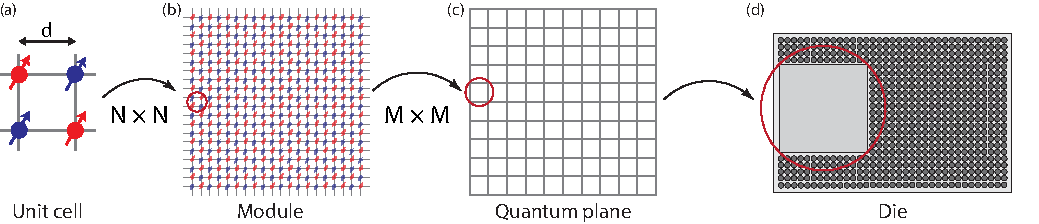
\includegraphics[width=0.98\textwidth]{Figure_1_array_schematic.pdf}
    \caption{Overview of the \textit{spider web} architecture with a schematic breakdown of its components, as described in the main text. (a) A unit cell contains four qubits that are separated by the qubit pitch \textit{d}. Qubits are colour coded to distinguish data qubits (blue) and ancilla qubits (red), as defined in the surface code. (b) A module constitutes of N$\times$N unit cells, and in turn M$\times$M modules together form (c) the quantum plane. Generally, the quantum plane occupies only part of (d) the die and the remaining area can be used to further reduce the off-chip wire count.}
    \label{fig:overview}
\end{figure*}

\textcolor{blue}{
  The overarching concept of the spider-web array is presented in \autoref{fig:unit_cell_schematics}.
  A large two-dimensional square-lattice of spin-qubits constitutes the \textit{quantum plane}.
  The spin-qubits consist of single electrons confined in electrostatically defined quantum dots in silicon.
  To implement the surface code~\cite{Dennis2002}, we assign qubits as data qubits or ancilla qubits in a chequerboard fashion, and allow single-qubit operations as well as nearest-neighbour two-qubit operations.   
  In contrast to most other spin-qubit architectures, this array is sparse, with a qubit pitch $d \sim 12$~\textmu m.
  This has two major implications:
  \begin{enumerate}
    \item It requires a non-conventional qubit operation protocol, which we implement by shuttling the qubits to operation regions--where single- and two-qubit operations are performed along with readout.
    \item It facilitates the local integration of classical control electronics, consisting here of sample-and-hold circuits that provide independent DC biasing of each gate electrode, which effectively offsets inhomogeneities in the potential landscape across the array.
    Consequently, the array can be considered fully homogeneous allowing the majority of qubit control signals to be shared across the entire array, which significantly reduces the number of control lines at the quantum plane boundary.
  \end{enumerate}
  The smallest operational set of elements contains of four qubits (\autoref{fig:overview}(a)).
  This \textit{unit cell} has an area of $(2d)^2$ and a perimeter of $8d$, and multiple unit cells can be concatenated to form a larger array.
  We define a \textit{module} \autoref{fig:overview}(b), consisting of $M = N \times N$ unit cells, with an area and a perimeter of $(2dN)^2$ and $8dN$, respectively.
  Modules define sections of the quantum plane where DC biasing and readout occur sequentially across the qubits in the module.
  Note that there can be different module sizes for DC biasing and readout ($M_b$ and $M_r$ respectively), and their size considerations will be discussed in the following sections.
  All other operations that are part of the surface code cycle occur simultaneously in all unit cells in the entire array.
  Completing the array, the quantum plane (\autoref{fig:overview}(c)) consist of \textit{M$\times$M} modules, covering an area and a perimeter of $(2dNM)^2$ and $8dNM$ respectively, with a total of $4M^2N^2$ qubits.
  As seen from \autoref{fig:overview}(d) the quantum plane does not occupy the entire area of the die, with the remaining space to be used to reduce the off-chip wire count even further. 
}

\begin{figure*}[t]
    \centering
    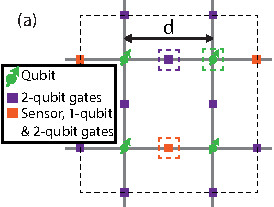
\includegraphics[height=0.225\textwidth,page=1]{Figure_2_unit_cell_schematic.pdf}
    \includegraphics[height=0.225\textwidth,page=2]{Figure_2_unit_cell_schematic.pdf}
    \includegraphics[height=0.225\textwidth,page=3]{Figure_2_unit_cell_schematic.pdf}
    \includegraphics[height=0.225\textwidth,page=4]{Figure_2_unit_cell_schematic.pdf}
    \caption{(a) Schematic (not to scale) of a unit cell containing four spin qubits (green), operations regions (purple/orange), connected via shuttling channels (grey lines). (b) Qubit idling region. Four barrier gate electrodes (red) define the confinement potential and allow qubits into the shuttling channels (defined by the blue gate electrodes). Cyan circles represent vias to higher interconnect layers. (c) Qubit operations region including control gates (red), sensing dot plunger (purple), source (S)/drain (D) ohmic contacts (squares) and micromagnets (orange rectangles). The gate electrodes labelled MW and J are used for single- and two-qubit operations (see main text), respectively. (d) Two-qubit operation only regions.}
    \label{fig:unit_cell_schematics}
\end{figure*}

\textcolor{blue}{
  A detailed schematic of the components of a unit cell is presented in \autoref{fig:unit_cell_schematics}.
  The unit cell mainly consists of large linear arrays of electrostatic gates, connecting the vertices of the qubit array to the operation regions (see \autoref{fig:unit_cell_schematics}(a)).
  The bulk of the gates in these linear arrays make up the shuttling channels (blue gates in \autoref{fig:unit_cell_schematics}).
  Four phase-shifted sinusoidal are applied to four consecutive gates (shades of blue in \autoref{fig:unit_cell_schematics}), creating a travelling-wave potential to trap and shuttle an electron.
  The shuttling signals are always on, and the sign of the phase difference between adjacent gates defines the shuttling direction.
  Four gates at the vertices of the spider-web array (red gates in \autoref{fig:unit_cell_schematics}(b), are used to control both the confinement potential that keeps the electrons at the vertex while idle, as well as the tunnelling in and out of the shuttling channels.
}
The qubits are shuttled to the operation regions between the vertices  in order to perform single- and two-qubit operations, as well as readout and initialization.
\textcolor{blue}{
  \autoref{fig:unit_cell_schematics}(c) shows a schematic of the gate structure used in the operation regions.  
  Single-qubit gates are performed via electric dipole spin resonance (EDSR) in a transverse magnetic field gradient provided by a pair of micromagnets~\cite{Pioro-Ladriere2007}.
  The native two-qubit operation is $\sqrt{SWAP}$, which relies on the exchange interaction between  electron spins~\cite{Loss1998,Divincenzo2000,Nielsen2016}.
  Qubit readout is performed via spin-to-charge conversion based on Pauli spin blockade~\cite{Zwanenburg2013}, using a charge sensing quantum dot connected to source/drain ohmic contacts.
  The array is initialized by loading electrons from the reservoirs and shuttling them to the vertices.
  Qubits are able to share an operation region to perform single-qubit gates and only ancilla qubits have to be read out, so not all operation regions require these capabilities.
  In contrast, two-qubit gates have to be performed between all qubit pairs.
  Therefore, as shown in \autoref{fig:unit_cell_schematics}(a), a unit cell contains four qubit idle regions (\autoref{fig:unit_cell_schematics}(b)), two regions to perform single- and two-qubit gates as well as initialization and readout (\autoref{fig:unit_cell_schematics}(c)), and six regions with a simpler gate structure, where only two-qubit gates can be performed (\autoref{fig:unit_cell_schematics}(d)).
  In the following section, we will describe in more detail the signals required on different gates to perform all of the operations in the spider-web array.
}

\subsection{Operation speeds}
\begin{itemize}
\item Fastest demonstrated  single(EDSR)- and two(exchange)-qubit operation times for Si quantum dot qubits.
\item Assuming 1 GHz shuttling signal and a gate pitch of 50 nm, the electrons will be shuttled with a velocity of 200 nm/ns and a distance of 10 \textmu m takes 50 ns.
\item Calculate the number of operations (and surface code cycles?) that can be achieved with typical(best) coherence times of Si qubits. 
\end{itemize}

\section{Electronics}\label{sec:electronics}
In this section we discuss the (local) electronics that is needed for DC biasing and for supplying the control signals for qubit operations, and to perform qubit readout.

\subsection{DC biasing}
To mitigate inhomogeneity in the qubit lattice, we design a sample-and-hold scheme to apply a local DC bias to the gate electrodes.
Based on the different gates functionalities, we define two bias voltage resolutions.
For gates acting as barriers to shuttling channels only a resolution sufficient to maintain an electron in a quantum dot is required and therefore we can afford a coarse resolution of 1~mV.
A resolution of 1 \textmu V is required for all other plunger and barrier gates~\cite{Vandersypen2017}.
To achieve the coarse resolution a minimum hold capacitance of $\sim$0.16 fF is required (limited by the electron charge $e/\Delta V$), while $\sim$14 pF (limited by thermal noise $k_B T/V^2$, assuming power dissipation from the local electronics raises the operating temperature to 1 K) is required for the fine resolution.
In the qubit idling region (\autoref{fig:unit_cell_schematics}(b)) the four barrier gates only require coarse resolution DC biasing.
In the qubit operation region shown in \autoref{fig:unit_cell_schematics}(c), a coarse resolution is sufficient for the two outer gates in the shuttling channel, while the seven other gates require a fine resolution.
In the two-qubit operation region (\autoref{fig:unit_cell_schematics}(d)), the three inner gates require a fine resolution, while for the two outer gates a coarse resolution is sufficient.
These requirements are summarized in Table~\ref{tab:DC_AC_count}.
A total of 64 control gates per unit cell require DC biasing, out of which 32 require fine resolution, while for the other 32 a coarse resolution is sufficient.
The need for DC biasing of the shuttling gates is eliminated by making the travelling wave potential large enough to overcome potential landscape inhomogeneities.

\begin{table}[b]
    \centering
    \begin{tabular}{l|c||c|c||c}
         & \# per & Fine & Coarse & Pulsed \\
         & unit cell & (1 $\mu$V) & (1 mV) & gates \\
        \hline \hline
        Qubit idling region & 4$\times$ & - & 4 & 4 \\
        \hline
        All-operation region & 2$\times$ & 7 & 2 & 6 \\
        \hline
        Two-qubit operations & 6$\times$ & 3 & 2 & 5 \\
        region & & & & \\
        \hline \hline
        Total per unit cell & & 32 & 32 & 58
    \end{tabular}
    \caption{Summary of the gates per unit cell requiring DC biasing and their resolution, and the number of pulsed signals.}
    \label{tab:DC_AC_count}
\end{table}

The DC biasing scheme is schematically depicted in \autoref{fig:dc_biasing_1}.
The open area in between the qubits and shuttling channels created by the sparseness of the \textit{spider web} array allows for local integration of demultiplexers and capacitors that together form sample-and-hold circuits.
Local demultiplexers (four per unit cell) each distribute DC voltages generated remotely (i.e. outside the quantum plane) to 16 local capacitors connected to the gate electrodes, by selecting one of their sixteen outputs based on a 4-bit address.

\begin{figure}[t]
    \centering
    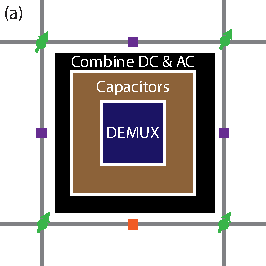
\includegraphics[height=0.2\textwidth,page=1]{Figure_3_DC_biasing_1.pdf}
    \includegraphics[height=0.2\textwidth,page=2]{Figure_3_DC_biasing_1.pdf}
    \caption{(a) Schematic of a unit cell containing locally integrated classical electronics. Demultiplexers in combination with capacitors form sample-and-hold-circuits to provide DC bias voltages. Additionally, circuits that combine the DC bias with AC control signals are required. (b) Input/output schematic of the demultiplexers. A demultiplexer (dark blue), once enabled via crossbar addressing (orange), ports the DC voltages coming from the sDAC (light blue) to the output selected by the 4-bit address bus (green). The dashed red line indicates the quantum plane boundary. The colour coding in (a) and the legend in (b) represent the same components in both panels as well as in Fig.\ref{fig:dc_biasing_2}.}
    \label{fig:dc_biasing_1}
\end{figure}

\begin{figure*}[t]
    \centering
    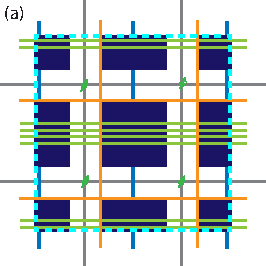
\includegraphics[height=0.275\textwidth,page=1]{Figure_4_DC_biasing_2.pdf}
    \includegraphics[height=0.275\textwidth,page=2]{Figure_4_DC_biasing_2.pdf}
    \includegraphics[height=0.275\textwidth,page=3]{Figure_4_DC_biasing_2.pdf}
    \caption{Schematics of (e) a unit cell and (d) a module. Demultiplexers are sequentially enabled by crossbar addressing controlled by multiplexers (orange blocks). (f) Schematic of the array of modules completing the quantum plane. Dashed red lines in (d) and (f) denote the quantum plane boundary.}
    \label{fig:dc_biasing_2}
\end{figure*}

\autoref{fig:dc_biasing_2} shows the DC biasing scheme on the unit cell, module and quantum plane levels.
All demultiplexers within a module share the same input DC biasing signal (\autoref{fig:dc_biasing_2}(b)), and all demultiplexers in the quantum plane share the same address bus (\autoref{fig:dc_biasing_2}(c)).
The demultiplexers in a module are enabled sequentially by crossbar addressing and in turn sequentially update each gate. This way, all modules are updated in parallel and therefore one module refresh cycle is required to refresh the entire qubit array.
The number of gates that can be updated sequentially will be limited by the required gate voltage refresh rate, that will be set by the current leakage of the hold circuit and the time required to update each gate.
This, in turn, will set the module size (i.e. the number of unit cells $N^2$ per module).

\subsection{Signals for qubit operations}

To perform single- and two-qubit operations, as well as readout and initialization, the qubits are shuttled to the operation regions in \autoref{fig:unit_cell_schematics}(c,d), where the operations are performed by applying pulsed signals to the appropriate gates.

Linear arrays of gate electrodes (blue gates in \autoref{fig:unit_cell_schematics}) define shuttling channels and a travelling wave potential can trap and shuttle an electron along these channels.
Four phase-shifted sinusoidal signals that are applied to four consecutive gates (different shades of blue in \autoref{fig:unit_cell_schematics}) and reused every \textcolor{red}{fourth} gate, are used to generate the travelling wave potential.
Electrons can be forced to tunnel into a shuttling channel by using a barrier gate (\autoref{fig:unit_cell_schematics}(b)).
The shuttling signals are always on and the phase shifts control the direction of shuttling.
The traveling wave potential is made large enough to overcome the inhomogeneities in the potential landscape, eliminating the need to apply DC biasing on the shuttling gates.
Electrons will travel the distance corresponding to four gate electrode in one period of the shuttling signal, so a 1 GHZ shuttling signal applied to the gates makes the electrons travel the distance corresponding to four gates per nanosecond.
Assuming a gate pitch of 50 nm, the electrons will be shuttled with a velocity of 200 nm/ns and a distance of 10 \textmu m takes 50 ns.

For single-qubit operations, a microwave pulse is applied to the control gate labelled MW in \autoref{fig:unit_cell_schematics}(c) in order to perform EDSR in the magnetic field gradient provided by a pair of micromagnets.
A pulsed signal to the gates labelled J in \autoref{fig:unit_cell_schematics}(c,d), that activates an exchange interaction between electrons underneath the adjacent gates, is used to perform a two-qubit operation.
\autoref{fig:dc+ac} schematically shows how AC signals for qubit operations are combined with DC biasing by employing a complementary switching circuit (see $\varphi_{AC}$ and $\overline{\varphi_{AC}}$).

All red gates in \autoref{fig:unit_cell_schematics}(b,d), and the five bottom gates and the gate labelled MW in \autoref{fig:unit_cell_schematics}(c) require pulsed signals.
This totals to 58 gates per unit cell requiring a pulsed signal, as summarised in the rightmost column of Table~\ref{tab:DC_AC_count}.

\begin{figure}[!b]
    \centering
    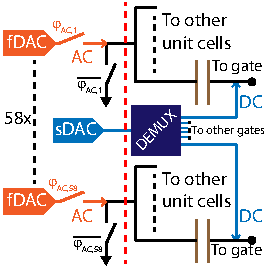
\includegraphics[height=0.35\textwidth]{Figure_5_DC-AC.pdf}
    \caption{Circuit schematic to combine AC and DC signals as described in the main text. fDAC (sDAC) are voltage sources for pulsed signals (DC biasing). The dashed red line indicates the quantum plane boundary.}
    \label{fig:dc+ac}
\end{figure}

\subsection{Readout}
Qubit readout is performed at the operation region shown in \autoref{fig:unit_cell_schematics}(c).
Charge sensing is done with a readout quantum dot connected to source/drain ohmic contacts and spin-to-charge conversion based on Pauli spin blockade is employed for spin readout~\cite{Zwanenburg2013}.
Additionally, the array is initialised by shuttling electrons that are provided by the ohmics in this operation region to the unit cell vertices.

Readout is performed sequentially across the unit cells of each module, while the modules are read out in parallel.
This is done by connecting the drain contacts of all sensor dots in a module to a single line at the quantum plane boundary and consecutively pulsing their plungers to bring them to the low-impedance, electrostatically sensitive regime, while all other sensor dots in the module are in Coulomb blockade (i.e. in the high-impedance regime).
A global readout demultiplexer is used for the sequential control of the sensor plungers in a module. This demultiplexer can be shared between all modules across the entire array.

Since qubit readout is the most time consuming operation and is performed sequentially within a module, it will most likely limit the surface code cycle rate as well as the ultimate size of the array.
Instead of using the same module size for both DC biasing and readout, we define readout modules that consist of $N_{RO}^2$ unit cells (with $N_{RO} \leq N$).
A total of $M_{RO}^2$ readout modules make up the full quantum plane (note: $NM = N_{RO}M_{RO}$).

Additionally, an extra level of parallel readout can be implemented by means of for example amplitude or frequency modulation.
Amplitude multiplexing can be achieved by tuning the DC bias of the sensor plungers that are read out at the same time to voltages that result in distinct amplitudes for the sensor response.
It is possible to use frequency multiplexing by using resonant circuits with different resonance frequencies.
Without going into details of the multiplexing strategy, we assume in the following four sensors to be read out simultaneously.
This does reduces the number of required sequential readouts and also slightly the number of lines. The latter, however, does not make a significant difference.

\section{Surface code operation}
\label{sec:surface_code}
The proposed array sustains the surface code by using a cyclic sequence of pulsed signals within a unit cell, with the same sequence performed in parallel across all unit cells in the entire array.
This is facilitated by the local DC biases, which allow to use the same control signals in all unit cells.
A total of 58 remote pulsed voltage sources are used to generate the required cyclic pulsed signals for all quantum control gates (i.e., one source per pulsed gate in a unit cell).

\autoref{fig:surface_code} depicts the surface code cycle. 
\autoref{fig:surface_code}(a) shows the circuit diagram for a single surface code cycle and is the 4-qubit analogue of the circuit shown in Ref.~\cite{Versluis2017}. For the present architecture only four qubits are required per unit cell, because the exchange coupling is not always present as is the case in superconducting qubits.
Steps 1--10 consist of either single- or two-qubit operations for which one or two of the qubits are shuttled from their idle position to the operation region to undergo either a single- or a two-qubit gate.
At the end of the cycle, the ancilla qubits are measured.
As an example, \autoref{fig:surface_code}(b,c) depict the qubit movement in steps 1 and 3, corresponding to single- and two-qubit gates, respectively.
%The qubit movement in the other steps is shown in the Supplementary Information.
Assuming both single- and two-qubit gates to take 100 ns to perform, a 1 GHz shuttling signal and 240 gates per lattice arm (see Sec.~\ref{sec:footprint}) each step of the surface code cycle takes ~160 ns.

\begin{figure}
    \centering
    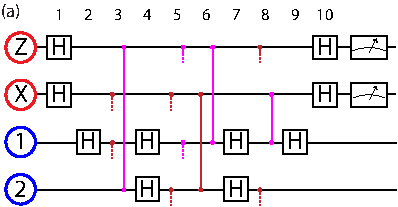
\includegraphics[width=86mm,page=1]{Figure_6_surface_code.pdf}\\
    \includegraphics[page=2]{Figure_6_surface_code.pdf}
    \includegraphics[page=4]{Figure_6_surface_code.pdf}
    \caption{Surface code operation of the spider web array. (a) Circuit diagram showing the surface code cycle for the four-qubit unit cell. H-blocks represent a Hadamard gate, solid lines represent a intra-unit cell two-qubit gates and dashed lines represent inter-unit cell two-qubit gates. (b,c) Schematics showing the qubit movement in step 1 (b) and step 3 (c) of the surface code cycle showing an example of single- and two-qubit gates respectively.}
    \label{fig:surface_code}
\end{figure}

Logic gates in the surface code with lattice surgery are achieved by creating defects in the lattice.
We implement these defects by preventing shuttling of a subset of data qubits via locally integrated switches.
The signals used to control these switches are arranged in a crossbar fashion across the entire quantum plane.
In practice, we propose to use $x$ crossbars over the entire array, in order to allow for $x$ defects to be simultaneously created and manipulated.
By activating a certain switch, the corresponding data qubit is not shuttled over to the operation region.
At the same time, the ancilla qubit with which the data qubit was supposed to have a two-qubit interaction is still shuttled over, but since the data qubit is not present, the two-qubit gate does not take place.

\section{Line scaling}
\label{sec:line_scaling}
The routing scheme for quantum control signals that we have described is summarized in Tab.~\ref{tab:routing}.
The outlined DC biasing scheme allows for significant sharing of control lines, which results in a very efficient scaling of ratio of the number of interconnects at the quantum plane boundary to the number of lines at the unit cell level.
The total number of gate electrodes at the unit cell level scales with number of qubits ($4M^2N^2$) and we will now discuss the scaling of the number of connections at the quantum plane boundary allowed by the operation schemes described before.
The line scaling at different levels of the spin qubit array for the control schemes described before is summarized in Table~\ref{tab:wire_count}.
A Rent’s exponent as low as $p=0.5$ is obtained at the quantum plane boundary.

\begin{table}[b]
    \centering
    \begin{tabular}{l|l}
        Shuttling gates & Source $\rightarrow$ gate  \\
        (blue) & \\
        \hline
        Pulsed gates & DC: source $\rightarrow$ local demultiplexer $\rightarrow$ gate \\
        (red) & AC: source $\rightarrow$ gate \\
        \hline
        Sensing dot & DC: source $\rightarrow$ local demultiplexer $\rightarrow$ gate \\
        plunger (purple) & AC: source $\rightarrow$ global demultiplexer $\rightarrow$ gate \\
        \hline
        Drain contacts & Measurement device $\leftarrow$ ohmic
    \end{tabular}
    \caption{Summary of signal routing for the four different type of control lines in the array design.}
    \label{tab:routing}
\end{table}

Independent DC biasing of the sparse array by means of sample-and-hold circuits is provided with $O(M^2+N)$ lines at the quantum plane boundary.
Concretely, at the unit cell level four digital address lines and four enabler line (two horizontal and two vertical) select a specific output of one demultiplexer, which is set to the correct voltage via a single connection to a voltage source.
This makes a total of nines line required for DC biasing, which all have to enter and leave the unit cell.
At the module level only the enabler lines scale with the number of unit cells as $4N$, that enter and leave the module.
Meanwhile, the four digital address lines and the connection to the voltage source is shared between all unit cells in a module. The digital address lines are common with other modules, so also have to leave the module.
Every module has its own voltage source, so at the quantum plane level $M^2$ connections to voltage sources are needed, while both the digital address lines and the enabler lines are shared between all modules.

\begin{table}[t]
    \centering
    \begin{tabular}{l|c|c|c}
         & Unit cell & Module & Quantum plane \\
        \hline \hline
        DC biasing & 18 & 8N+9 & M\textsuperscript{2}+4N+4 \\
        \hline
        Shuttling & 8 & 8 & 4 \\
        \hline
        Pulsed signals & 116 & 116 & 58 \\
        \& MW & & & \\
        \hline
        Logical & 8x & 8Nx & 4NMx \\
        operations & & & \\
        \hline
        Readout & 4 & 4$\log_2 N_{RO}-1$ & $M_{RO}^{2}+$ \\
        & & & $2\log_2 N_{RO}-1$ \\
        \hline \hline
        & 146+8x & 8N(1+x)+ & $M^{2} + M_{RO}^{2}$ \\
        Total & & 4$\log_2 N_{RO}$+132 & +4N(1+Mx) \\
        & & & +2$\log_2 N_{RO}$+65
    \end{tabular}
    \caption{Line scaling at different levels of the array. At the unit cell and module level most lines are counted double, since they have to enter and leave through the perimeter.}
    \label{tab:wire_count}
\end{table}

Shuttling of electrons across the array only requires four signals that can be fully shared over the entire array.
At the unit cell and module level these connection have to enter and leave, so they count double.

A constant number of 58 lines (see Tab.~\ref{tab:DC_AC_count}) at the quantum plane boundary (irrespective of the number of qubits) suffices to sustain the surface code by delivering all pulsed and microwave control signals across the entire chip.
These lines are counted double at the unit cell and module level, as they enter and leave.

Switches are used to deactivate data qubits in order to implement logical operations in the surface code.
The signals to control those switches are arranged in a crossbar fashion over the entire quantum plane with as few as $O(xMN)$ lines.
A total of $x$ defects can be created and manipulated simultaneously by $x$ parallel crossbars over the entire array.
For every crossbar, two horizontal and two vertical lines have to enter and leave a unit cell and this scales with $N$ and $NM$ at the module and quantum plane level, respectively.
The lines enter and leave at the unit cell and module level, so are counted double.

Decoding is used to address the sensor plungers in a readout module for the sequential readout scheme and it thereby obtains a line scaling at the quantum plane boundary as $O(M_{RO}^2+\log(N_{RO}))$.
A unit cell contains two readout SETs that both require a connection to their plunger and share a single ohmic line that has to enter and leave the unit cell.
At the module level a single ohmic line is required to enter, and $2\log_2 N_{RO}-1$ lines enter and leave the module to address the readout demultiplexers, assuming four plungers to be connected to a single line for multiplexed readout.
To read out the full quantum plane, all $M_{RO}^2$ modules require their own ohmic line, while the address lines for the readout demultiplexer are shared.

The wire count at different levels of the array does depend on the total number of qubits, but also on the exact choice of the module size $N$ and the corresponding value for $M$ (for a given total number of qubits), as well as the number of parallel crossbars for lattice surgery.
Assuming a total of $2^{20}$ ($\approx10^6$) qubits to make a concrete assessment of the number of lines, a module size of $N = 2^6 = 64$ requires $M = 2^3 = 8$ modules.
For the sake of this example we assume $x=32$ parallel crossbars.
The number of connections for this choice of $N$, $M$ and $x$ is summarized in Tab.~\ref{tab:wire_count_example}.
With a qubit pitch $d=$12 \textmu m (see next section) and these numbers for $N$ and $M$, a unit cell, module and the quantum plane have a perimeter of $8d\approx$ 96 \textmu m, $8dN\approx$ 12 mm and $8dNM\approx$ 49 mm, respectively.
\textcolor{red}{The line density is highest at the unit cell level where $O(10^2-10^3)$ wires pass through the unit cell perimeter, using multiple interconnect layers.
}

\begin{table}[t]
    \centering
    \begin{tabular}{l|c|c|c}
         & Unit cell & Module & Quantum plane \\
        \hline \hline
        DC biasing & 18 & 8N+9 & M\textsuperscript{2}+4N+4 \\
        \hline
        Shuttling & 8 & 8 & 4 \\
        \hline
        Pulsed signals & 116 & 116 & 58 \\
        \& MW & & & \\
        \hline
        Logical & 8x & 8Nx & 4NMx \\
        operations & & & \\
        \hline
        Readout & 4 & 4$\log_2 N_{RO}-1$ & $M_{RO}^{2}+$ \\
        & & & $2\log_2 N_{RO}-1$ \\
        \hline \hline
        & 146+8x & 8N(1+x)+ & $M^{2} + M_{RO}^{2}$ \\
        Total & & 4$\log_2 N_{RO}$+132 & +4N(1+Mx) \\
        & & & +2$\log_2 N_{RO}$+65
    \end{tabular}
    \caption{\textcolor{red}{TO BE UPDATED - }Number of connections at different levels of the array and for different purposes for $N=64$, $M=8$ and $x=32$.}
    \label{tab:wire_count_example}
\end{table}

\section{Footprint}
\label{sec:footprint}
Next, we make an assessment of the footprint of the classical control electronics we have discussed before.
Since this electronics has to be integrated locally, the corresponding footprint set the qubit pitch $d$.
The most significant contribution to the footprint comes from the capacitors that are required for the sample-and-hold scheme.
As summarized in Tab.~\ref{tab:DC_AC_count}, a total of 32 gate electrodes per unit cell require a fine voltage resolution and for another 32 gate electrodes a coarse voltage resolution is sufficient.
The total capacitance per unit cell therefore is $\sim$450 pF.
State-of-the-art deep-trench capacitor technology achieves $\sim$1 pF/\textmu m\textsuperscript{2}~\cite{Park2015}, so we estimate a total capacitor footprint of $\sim$450 \textmu m\textsuperscript{2}.
In order to estimate the footprint for the demultiplexers used for DC biasing and readout, we extrapolate to 28-nm technology from a modelled demultiplexer circuit in 40-nm technology.
We obtain an estimate of the total footprint of the DC biasing and readout demultiplexers of $\sim$60 \textmu m\textsuperscript{2} per unit cell.
The total footprint of the classical control electronics per unit cell therefore is $\sim$510 \textmu m\textsuperscript{2}.
This allows to set the qubit pitch to d$\geq$12 \textmu m and results in a unit cell area of $4d^2=$ 576 \textmu m\textsuperscript{2}.
With a 50-nm gate pitch, each of the lattice arms would comprise 240 gate electrodes.

For a concrete assessment of the footprint of the array design discussed here, let us again consider a total of $(2MN)^2 = 2^{20}$ ($\approx10^6$) qubits.
A total area of $(2dNM)^2\approx$151 mm\textsuperscript{2} is covered by the quantum plane.
The remaining area on, for example, a typical 22 mm $\times$ 33 mm (726 mm\textsuperscript{2}) die is $\sim$575 mm\textsuperscript{2}, and can be used to implement classical control circuits, i.e. among others the pulsed voltage sources we have described.
In addition, additional levels of multiplexing can be employed to bring the off-chip wire count, typically being the real bottleneck for Rent’s rule, to well below the wire count at the quantum plane boundary.

\textcolor{orange}{We now consider the footprint requirements of the control electronics that need to be locally integrated in the quantum plane, which sets the qubit pitch $d$.
%and the wire density at various levels.
The bulk of the footprint will be taken up by the capacitors required for the sample-and-hold scheme.
Coarse resolution is required for 32 gates and another 32 gates require fine resolution, which comprise a total capacitance per unit cell of $\sim$450 pF. 
Assuming $\sim$1 pF/$\mu$m\textsuperscript{2} (using state-of-the-art deep-trench capacitor technology~\cite{Park2015}), we estimate a total capacitor footprint of $\sim$450 $\mu$m\textsuperscript{2}.
In addition, we modelled a demultiplexer circuit using 40-nm technology, extrapolated to 28-nm technology and obtained an estimate of the total footprint of the DC biasing and readout demultiplexers of $\sim$60 $\mu$m\textsuperscript{2} per unit cell.
This adds to a total footprint per unit cell of $\sim$510 $\mu$m\textsuperscript{2}, which allows to set the qubit pitch to d$\geq$12 $\mu$m.
Assuming a 50 nm pitch between gate electrodes, this would require linear arrays of 240 gate electrodes per lattice arm.
A unit cell has an area of $4d^2\approx576 \,\mu$m\textsuperscript{2}.%, $(2dN)^2$ and $(2dNM)^2$, respectively.
}

\textcolor{orange}{In order to make a concrete assessment of the feasibility of the proposed design and scheme let us assume a total of $(2MN)^2 = 2^{20}$ qubits.
The total area covered by the quantum plane is $(2dNM)^2\sim$151 mm\textsuperscript{2}.
The remaining area on a typical 22 mm $\times$ 33 mm (726 mm\textsuperscript{2}) die is $\sim$575 mm\textsuperscript{2}, and can be used to implement classical control circuits and to bring the wire count going off-chip, typically the real bottleneck for Rent’s rule, to well below the wire count at the quantum plane boundary by means of additional levels of multiplexing.
}


\section{Capacitance and heat load?}













%%% Acknowledgments

\begin{acknowledgments}

\end{acknowledgments}

%%% References
\bibliographystyle{apsrev4-1}
\bibliography{references}

\end{document}